\section{Validierung}
\vspace{0.5cm}
Um das implementierte Tool zu testen, wurde eine virtuelle Maschine verwendet. Hierfür war es zunächst notwendig, die Virtualisierungssoftware VirtualBox \footnote{Download unter \url{https://www.chip.de/downloads/VirtualBox_23814448.html}, zuletzt verfügbar am 16.06.2020}  herunterzuladen. Im Anschluss war es möglich, bei Microsoft einen bereits fertigen Evaluierungscomputer als virtuelle Maschine (VM) mit Windows 10 \footnote{Download unter \url{https://developer.microsoft.com/de-de/windows/downloads/virtual-machines/}, zuletzt verfügbar am 16.06.2020}  herunterzuladen. Diese VM konnte nach dem Entpacken problemlos in VirtualBox importiert und ausgeführt werden. Nach der Installation der Gasterweiterungen \footnote{Download unter \url{http://download.virtualbox.org/virtualbox/}, zuletzt verfügbar am 16.06.2020} wurde ein gemeinsamer Ordner festgelegt, mit dem ein Datenaustausch zwischen dem Gast- und Host-System möglich ist, um das selbst implementierte Tool auch in der VM starten zu können. \\
\\
Um zu testen, ob das Tool eine korrekte Auswertung der ShellBag-Informationen vornimmt, wurde im Folgenden eine Testreihe durchgeführt. Zunächst wurde die SID des aktuell angemeldeten Benutzers mit dem Befehl \glqq \texttt{whoami /user}\grqq{} in der Eingabeaufforderung bestimmt, um im Tool den richtigen Benutzer auszuwählen. Die SID des aktuell angemeldeten Benutzers \texttt{windev2004eval$\backslash$user} lautete \texttt{S-1-5-21-3234566417-3121902272-2793192418-1001}. 

Da während der Installation und Konfiguration der virtuellen Maschine bereits ShellBag-Informationen entstanden sind, wurden zunächst die aktuellen ShellBag-Informationen des Benutzers im Tool ausgegeben und in der nachfolgenden Abbildung \ref{img:vorher} festgehalten. 

\begin{figure}[H]
	\centering
	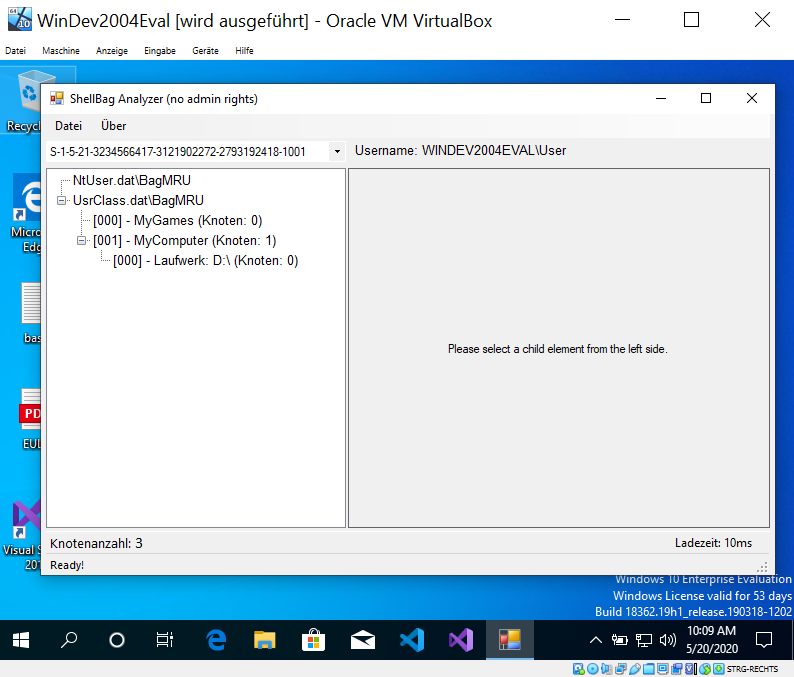
\includegraphics[width=0.8\textwidth]{part/vorher.png}
	\caption{ShellBag-Einträge vor der Testreihe} 
	\label{img:vorher}
\end{figure}

Basierend auf diesem Ergebnis wurde nun eine Testreihe aufgestellt und eine erneute Auswertung im Tool vorgenommen. Die nachfolgende Tabelle \ref{akt} zeigt die durchgeführten Aktivitäten mit den entsprechenden Zeitangaben. Diese Zeiten wurden entsprechend in der Systemsteuerung eingestellt.

\begin{longtable}{|p{0.3\textwidth}|p{0.6\textwidth}|}
	\caption{Testreihe für Ordneraktivitäten} \label{akt} \vspace{1em} \\
	\hline
	\cellcolor{gray!25}\textbf{Zeit} & \cellcolor{gray!25}\textbf{Aktivität} \\
	\hline
    20.05.2020 10:11 Uhr & Anlegen eines Ordners \glqq test\grqq{} auf dem Desktop \\
	\hline
	20.05.2020 10:12 Uhr & Öffnen und Schließen des Ordners \glqq test\grqq{} \\
	\hline
	20.05.2020 10:13 Uhr & Anlegen eines ZIP-komprimierten Ordners \glqq studium\grqq{} auf dem Desktop \\
	\hline
	20.05.2020 10:15 Uhr & Öffnen und Schließen des ZIP-komprimierten Ordners \glqq studium\grqq{} \\
	\hline
	20.05.2020 10:16 Uhr & Anlegen eines Unterordners \glqq softwareprojekt\grqq{} unter \glqq test\grqq{} \\
	\hline
	20.05.2020 10:18 Uhr & Öffnen und Schließen des Unterordners \glqq softwareprojekt\grqq{} \\
	\hline
	20.05.2020 10:19 Uhr & Öffnen des Laufwerkes C:$\backslash$ im Datei-Explorer unter \glqq My Computer\grqq{}\\
	\hline
\end{longtable}
\vspace{1em}

Zunächst wurde die Ausgabe im Tool mit der Ausgabe im Registrierungs-Editor verglichen, um zu überprüfen, ob die Struktur der ShellBags korrekt übernommen wurde. Die nachfolgenden Abbildungen \ref{img:regedit} und \ref{img:nachher} zeigen einen Ausschnitt. 

\begin{figure}[H]
	\centering
	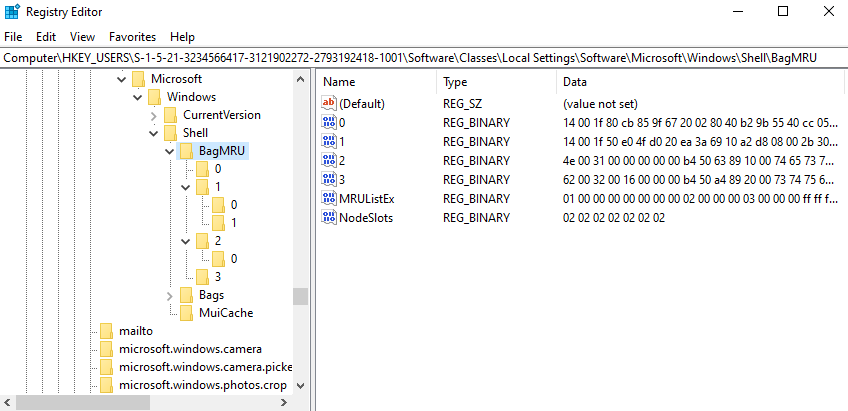
\includegraphics[width=0.8\textwidth]{part/regedit.png}
	\caption{ShellBag-Baumstruktur im Registrierungs-Editor nach der Testreihe} 
	\label{img:regedit}
\end{figure}

\begin{figure}[H]
	\centering
	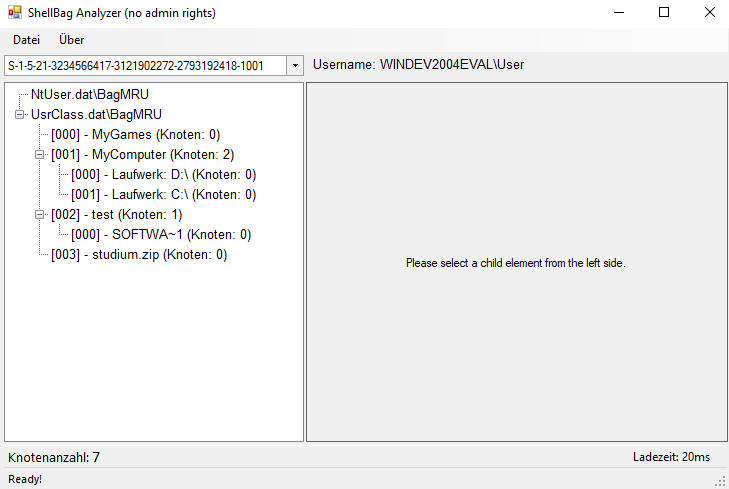
\includegraphics[width=0.8\textwidth]{part/nachher.png}
	\caption{ShellBag-Baumstruktur im Tool nach der Testreihe} 
	\label{img:nachher}
\end{figure}

Wie zu erkennen ist, sind die beiden Strukturen identisch. Die ShellBag-Struktur wurde somit korrekt im Tool abgebildet. 

Im Anschluss erfolgte ein Abgleich der Daten im rechten Fenster, in dem alle Informationen eines Values in einer lesbaren Form dargestellt werden. 

Der Ordner \glqq test\grqq{} wurde als Subkey unter BagMRU angelegt und entspricht einem File Entry Shell Item mit dem Class Type Indicator von 0x31. Dies wurde korrekt im rechten Fenster erfasst. Auch der Primary- und Secondary Name wurde korrekt abgebildet. Die Extension Version lautet 0x0009, welche für Windows 10 steht. Alle drei Zeitstempel wurden ebenfalls korrekt umgewandelt. Es bleibt anzumerken, dass es sich hierbei um die UTC-Zeit handelt. Da in der virtuellen Maschine als Zeitzone die Pacific Time (UTC-8:00) eingestellt ist, müssen zu den in Tabelle \ref{akt} abgebildeten Zeiten durch die aktuelle Sommerzeit sieben Stunden hinzuaddiert werden, um die koordinierte Weltzeit zu erhalten \cite{zz}. Auch diese Zeit wurde im Tool korrekt abgebildet. 

Der Subkey des ZIP-komprimierten Ordners \glqq studium\grqq{} wurde ebenfalls unter BagMRU angelegt. Auch hier wurden die Informationen korrekt dargestellt. Im Unterschied zu einem normalen Ordner besitzt der ZIP-komprimierte Ordner den Class Type Indicator von 0x32. Diese Unterscheidung wird vom Tool ebenfalls erfasst. 

Der Eintrag zum Unterordner \glqq softwareprojekt\grqq{} wurde korrekt als Subsubkey unter dem Subkey, der für den Ordner \glqq test\grqq{} steht, angelegt. Auch diese Informationen des File Entry Shell Items wurden korrekt dargestellt. Der Primary Name wurde im Long File Name Format \glqq SOFTWA\raisebox{-0.9ex}{\~{}}1\grqq{} gespeichert. Im Secondary Name ist der vollständige Name abgelegt.

Das Öffnen des Laufwerkes C:$\backslash$ führte in den ShellBags dazu, dass unter dem Subkey, der für \glqq My Computer\grqq{} steht, ein Subkey angelegt wurde. Das Laufwerk repräsentiert ein Volume Shell Item mit dem Class Type Indicator von 0x2F. Diese Information war im rechten Fenster sichtbar, genau wie der Laufwerksbuchstabe.

Der übergeordnete Knoten des Laufwerkes C:$\backslash$ steht für das Root Folder Shell Item \glqq My Computer\grqq{} mit dem Class Type Indicator von 0x1F und dem Sort Index von 0x50. Dieser Eintrag war bereits vor der Testreihe durch vorher getätigte Einstellungen vorhanden. Es konnte somit jedoch bestätigt werden, dass es sich tatsächlich um den standardmäßig vorhandenen Ordner handelt, da das Laufwerk geöffnet wurde, indem zuvor auf \glqq My Computer\grqq{} geklickt wurde. Die GUID des Root Folder Shell Items wurde ebenfalls korrekt dargestellt. Diese lautet \texttt{20d04fe0-3aea-1069-a2d8-08002b30309d}.

Es konnte somit festgestellt werden, dass die Baumstruktur korrekt aus der Registry übernommen wurde und alle Informationen der jeweiligen Shell Items korrekt abgebildet und interpretiert wurden. \\
\\
Außerdem kann die Ladezeit betrachtet werden. Diese gibt an, welche Zeitdauer das Tool benötigt hat, um die ShellBag-Einträge auszuwerten und darzustellen. In diesem Fall benötigte das Tool 20 ms für 7 ShellBag-Einträge. Dies entspricht im Durchschnitt ca. 2,86 ms pro Eintrag. \\
\\
Nun wurde die im Tool integrierte Export-Funktion getestet. Dafür wurden die im Tool ausgegebenen ShellBag-Einträge der Testreihe exportiert. Es wurde jeweils eine .TXT-Datei für ShellBags der NTUSER.dat und der USRCLASS.dat im Verzeichnis, in dem die ausführbare Datei liegt, gespeichert. Diese Dateien wurden mit einem Editor geöffnet. Wie bereits im Tool erkennbar war, gab es für die Testreihe keine Einträge in der NTUSER.dat. Aus diesem Grund ist die Datei leer. Die Datei der USRCLASS.dat beinhaltet jedoch alle ShellBag-Einträge, die im Tool aufgrund der Testreihe ausgegeben wurden. Auch hier wurden die Informationen vollständig und in einer hierarchischen Struktur abgebildet. Die nachfolgende Abbildung \ref{img:export} zeigt den Ausschnitt der Datei. 

\begin{figure}[H]
	\centering
	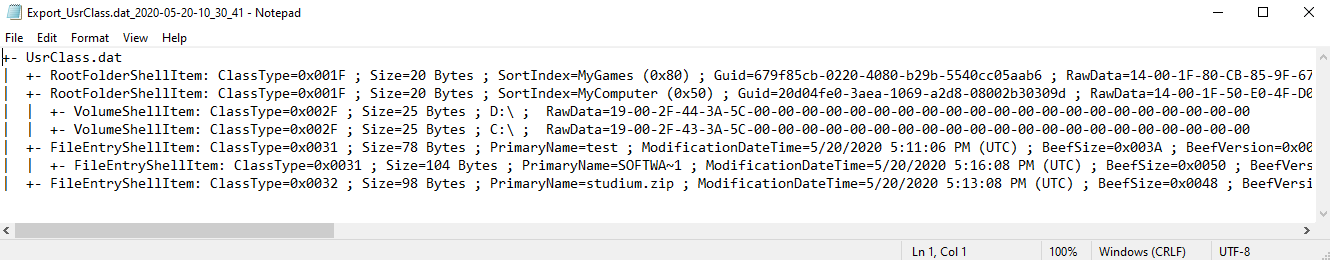
\includegraphics[width=1\textwidth]{part/export.png}
	\caption{Ausschnitt der Datei mit exportierten ShellBag-Einträgen der USRCLASS.dat} 
	\label{img:export}
\end{figure}


